%% IFBTcc Latex Template Version
%% 	based on a fork of : RiSE Latex Template
%%
%% IFBthesis latex template for thesis and dissertations
%% https://github.com/IFBmodels/tcc
%%
%% (c) 2017 Rafael de Campos Passos (rcpassos@ieee.org)
%%
%% This document was initially based on RiSE Latex template, from Yguaratã
%% Cerqueira Cavalcanti
%%
%% GENERAL INSTRUCTIONS
%%
%% We strongly recommend you to compile your documents using pdflatex command.
%% It is also recommend use the texlipse plugin for Eclipse to edit your documents.
%%
%% Options for \documentclass command:
%%         * Idiom
%%           pt   - Portguese (default)
%%           en   - English
%%
%%         * Text type
%%           bsc  - B.Sc. Thesis
%%           msc  - M.Sc. Thesis (default)
%%           qual - PHD qualification (not tested yet)
%%           prop - PHD proposal (not tested yet)
%%           phd  - PHD thesis
%%
%%         * Media
%%           scr  - to eletronic version (PDF) / see the users guide
%%
%%         * Pagination
%%           oneside - unique face press
%%           twoside - two faces press
%%
%%		   * Line spacing
%%           singlespacing  - the same as using \linespread{1}
%%           onehalfspacing - the same as using \linespread{1.3}
%%           doublespacing  - the same as using \linespread{1.6}
%%
%% Reference commands. Use the following commands to make references in your
%% text:
%%          \figref  -- for Figure reference
%%          \tabref  -- for Table reference
%%          \eqnref  -- for equation reference
%%          \chapref -- for chapter reference
%%          \secref  -- for section reference
%%          \appref  -- for appendix reference
%%          \axiref  -- for axiom reference
%%          \conjref -- for conjecture reference
%%          \defref  -- for definition reference
%%          \lemref  -- for lemma reference
%%          \theoref -- for theorem reference
%%          \corref  -- for corollary reference
%%          \propref -- for proprosition reference
%%          \pgref   -- for page reference
%%
%%          Example: See \chapref{chap:introduction}. It will produce
%%                   'See Chapter 1', in case of English language.
%%
%% Citation commands:
%%          \citet (from natbib) -- To cite a reference as part of the narrative
%%          \citep (from natbib) -- To cite a reference between parenthesis
%%          citationblock environment -- To produce direct citation blocks according to the ABNT

\documentclass[pt,twoside,onehalfspacing,bsc]{ifbclass/ifbclass}

  \usepackage{colortbl}
  \usepackage{color}
  \usepackage[table]{xcolor}
  \usepackage{microtype}
  \usepackage{bibentry}
  \usepackage{subfigure}
  \usepackage{multirow}
  \usepackage{rotating}
  \usepackage{booktabs}
  \usepackage{pdfpages}
  \usepackage{caption}
  \usepackage{lipsum}
  \usepackage{sectsty}
  
  %% Set the language used in your code in the block above
  
  \captionsetup[table]{position=top,justification=centering,width=.85\textwidth,labelfont=bf,font=footnotesize}
  \captionsetup[lstlisting]{position=top,justification=centering,width=.85\textwidth,labelfont=bf,font=footnotesize}
  \captionsetup[figure]{position=bottom,justification=centering,width=.85\textwidth,labelfont=bf,font=footnotesize}
  
  %% Chapter and (Sub)Section fonts must be same size as text (12)
  \sectionfont{\fontsize{12}{15}\selectfont}
  \subsectionfont{\fontsize{12}{15}\selectfont}
  \subsubsectionfont{\fontsize{12}{15}\selectfont}
  
  %% Change the following pdf author attribute name to your name.
  \usepackage[linkcolor=black,
              citecolor=black,
              urlcolor=black,
              colorlinks,
              pdfpagelabels,
              pdftitle={Rise Thesis Template (ABNT)},
              pdfauthor={Rise Thesis Template (ABNT)},
              breaklinks=true]{hyperref}
  
  \address{BRASÍLIA}
  
  \universitypt{Instituto Federal de Brasília}
  \universityen{Federal Institute of Brasilia}
  
  \campus{Campus Taguatinga}
  
  \departmentpt{Departamento de Computação}
  \departmenten{Computer Department}
  
  \programpt{Bacharelado em Ciência da Computação}
  \programen{Bachelors in Computer Science}
  
  \majorfieldpt{Ciência da Computação}
  \majorfielden{Computer Science}
  
  \title{Título do Trabalho }
  
  \date{2017}
  
  \author{Nome completo do Autor}
  \adviser{Nome completo do Orientador}
  \coadviser{Nome dompleto do co-orientador }
  
  % Macros (defines your own macros here, if needed)
  \def\x{\checkmark}
  %\let\lstlistoflistings\origlstoflistings
  \begin{document}
  
  \frontmatter
  
  \frontpage
  
  \presentationpage
  
  \begin{fichacatalografica}
    \FakeFichaCatalografica % Comment this line when you have the correct file
  %     \includepdf{fig_ficha_catalografica.pdf} % Uncomment this
  \end{fichacatalografica}
  
  \banca
  
  \begin{dedicatory}
  I dedicate this thesis to all my family, friends and professors who gave me the
  necessary support to get here.
  \end{dedicatory}
  
  \acknowledgements
  \input{text/agradecimentos}
  
  \begin{epigraph}[]{Márcio de Deus}
  When one finds a hard problem, the more complicated it is, the more one ought to work towards enlightening it's solution.
  \end{epigraph}
  
  \resumo
  % Escreva seu resumo no arquivo resumo.tex
  {\parindent0pt
    \input{text/resumo}
  }
  
  \abstract
  % Write your abstract in a file called abstract.tex
  {\parindent0pt
    \input{text/abstract}
  }
  
  % List of figures
  \listoffigures
  
  % List of Codes
  \lstlistoflistings
  
  % List of tables
  \listoftables
  
  % List of acronyms
  % Acronyms manual: http://linorg.usp.br/CTAN/macros/latex/contrib/acronym/acronym.pdf
  \listofacronyms
  \input{text/acronyms}
  
  % Summary (tables of contents)
  \tableofcontents
  
  \mainmatter
  
  \include{text/introduction}
  \include{text/background}
  \chapter{Development}

\section{Convolução e Convolução Discreta}
Em matemática, a convolução é um operador linear aplicado em duas funções. 
Uma operador linear, é um caso especifico de uma transformação linear, que por sua vez também pode ser chamada por mapeamento linear ou função linear, é uma operação que, dados os conjuntos não vazios $A$ e $B$, o mapeamento $f$ de $A$ para $B$ é denotador por $f : A \to B$ onde $A$ representa o domínio e $B$ representa a imagem.
Para um mapeamento dos espaços vetorias $A$ e $B$ sobre o mesmo corpo $C$ ser considerado linear, ele deve preservar as operações de adição vetorial e multiplicação por escalar. 
Ou seja, deve cumprir as seguinte condições:\\
(1) para qualquer vetor $a, a' \in A$, $f(a+a') = f(a) + f(a')$\\
(2) para qualquer número escalar $e$ e vetor $a \in A$, $f(ka) = kf(a)$\\
No caso especifico do operador linear, esta transformação deve ocorrer dentro de um mesmo espaço vetorial.
Ou seja, uma transformação $f$ em um espaço vetorial $A$ sobre um corpo $C$ representada por $f : A \to A$.
\citep{lipschutz2009linear} \\%\par
Dadas as definições anteriores, um operador linear $f$ em um espaço vetorial $R^2$, $f : R^2 \to R^2$, definido por $f(x,y) \to (x,-y)$, operando em cima de um vetor $a \in R^2$ tal que $a = (1,1)$, resulta em uma imagem de $a' = (1,-1)$, representados respectivamente pela linha azul e vermelha na figura \ref{fig:operacaolinear}.
\begin{figure}[h] 
  \centering
  \caption[Transformação Linear $f(x,y) \to (x,-y)$]{Transformação Linear $f(x,y) \to (x,-y)$}
    \label{fig:operacaolinear}
    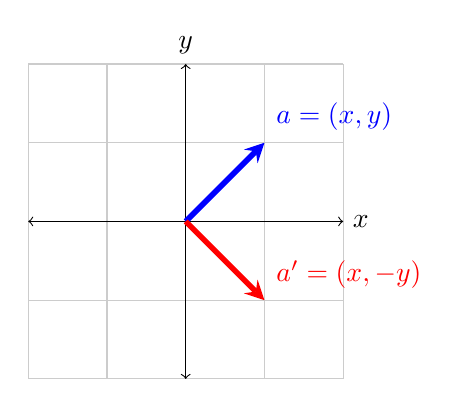
\begin{tikzpicture}
        \draw[thin,gray!40] (-2,-2) grid (2,2);
        \draw[<->] (-2,0)--(2,0) node[right]{$x$};
        \draw[<->] (0,-2)--(0,2) node[above]{$y$};
        \draw[line width=2pt,blue,-stealth](0,0)--(1,1) node[anchor=south west]{$\boldsymbol{a = (x,y)}$};
        \draw[line width=2pt,red,-stealth](0,0)--(1,-1) node[anchor=south west]{$\boldsymbol{a' = (x,-y)}$};
      \end{tikzpicture}
\end{figure}
Essa operação também pode ser representada de forma matricial. A transformação linear anteriormente denotada por $f(a)$ pode ser descrita pelo produto matricial da matriz de transformação $T : R^2 \in R^2$ pelo vetor $v$ tal que $v \in R^2$ da seguinte forma:
$$T = \begin{bmatrix}1 && 0 \\ 0 && -1\end{bmatrix} v = \begin{bmatrix}x \\ y\end{bmatrix}$$ 
$$T\cdot v = \begin{bmatrix}1 && 0 \\ 0 && -1\end{bmatrix}\begin{bmatrix}x \\ y\end{bmatrix} = \begin{bmatrix}x \\ -y\end{bmatrix}$$
Com os valores do vetor $v$ equivalentes ao vetor $a = (1,1)$ do exemplo anterior, temos a operação linear:
$$\begin{bmatrix}1 && 0 \\ 0 && -1\end{bmatrix}\begin{bmatrix}1 \\ 1\end{bmatrix} = \begin{bmatrix}1 \\ -1\end{bmatrix}$$






e produz uma terceira função que representa ... A convolução é uma operação matemática com aplicações em vários temas, e principalmente em processamento de sinais.


% \section{Introduction}

% \lipsum[1]

% \begin{code}[language=Python,caption=Python Fribonacci Code,label=code:frib]
% from math import *

% # define function
% def analytic_fibonacci(n):
%   sqrt_5 = sqrt(5);
%   p = (1 + sqrt_5) / 2;
%   q = 1/p;
%   return int( (p**n + q**n) / sqrt_5 + 0.5 )

% for i in range(1,31):
%   print analytic_fibonacci(i)
% \end{code}


% This is a reference to Code \ref{code:frib} \ldots{}

% \lipsum[1]

% \begin{code}[language=C,caption=Hello World C Code,label=code:helloc]
% #include<stdio.h>

% main()
%     {
%         printf("Hello World");
%     }
% \end{code}


% This is a reference to Code \ref{code:helloc} \ldots{}

% \lipsum[1]

% \begin{code}[language=Java,caption=Hello Java Code,label=code:helloj]
% public class HelloWorld {

%     public static void main(String[] args) {
%         System.out.println("Hello, World");
%     }
% }
% \end{code}


% This is a reference to Code \ref{code:helloj} \ldots{}


% \section{Section}

% \lipsum[2-4]

% \subsection{Subsection}

% \lipsum[2-4]

  \include{text/conclusion}
  
  % References
  
  \begin{references}
    \bibliography{bib/references}
  \end{references}
  
  % Appendix
  
  \theappendix
  \include{appendix/mapping-study}
  
  \end{document}
  